% !TeX program = pdflatex
\documentclass[tikz,border=8pt]{standalone}
\usepackage{pgfplots}\pgfplotsset{compat=1.16}
\definecolor{FigureBlue}{HTML}{2563EB}\definecolor{FigureOrange}{HTML}{EA580C}
\begin{document}
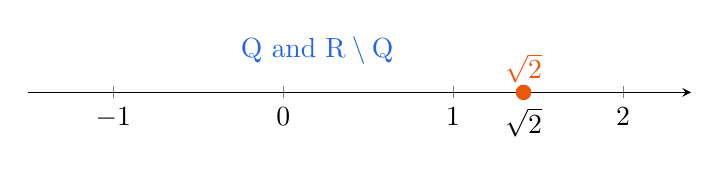
\begin{tikzpicture}
\begin{axis}[width=10cm,height=2.4cm,axis y line=none,axis x line=middle,xmin=-1.5,xmax=2.4,ymin=-.4,ymax=.6,xtick={-1,0,1,1.41421356,2},xticklabels={$-1$,$0$,$1$,$\sqrt2$,$2$},ytick=\empty,clip=false]
  \addplot[only marks,mark=*,mark size=2.6pt,FigureOrange] coordinates {(1.41421356,0)};
  \node[FigureOrange,above] at (axis cs:1.41421356,0) {$\sqrt2$};
  \node[FigureBlue,above] at (axis cs:.2,.28) {$\mathrm{Q}$ and $\mathrm{R}\setminus\mathrm{Q}$};
\end{axis}
\end{tikzpicture}
\end{document}
